\section*{Introduction}
\label{sec:introduction}

\revise{A fundamental challenge that brains face is to extract relevant information
from high-dimensional external stimuli
that forms the neural basis of an organism's decision making
and interaction with the world.}

Brains face the fundamental challenge of
\revise{extracting relevant information from high-dimensional external stimuli
in order to form the neural basis 
that guides an organism's behavior and interaction with the world.

using patterns of neural activity
in order to allow an organism to interact with the world.}
% Brains face the fundamental challenge of 
% processing, storing, and representing high-dimensional stimuli
% using patterns of neural activity \revise{that propagate behaviorally relevant information about the environment across regions}.
% \mikeNote{R1: The authors seem to subconsciously imply that they see their model as more relevant for the sensory system, based on a number of statements they make in parts of the paper that are supposed to be more general. For example: 1) Lines 2-3: The sentence that sets up the paper already takes a sensory view; the authors don’t say anything about interacting with the world; 2) Lines 73-4; 3) Lines 290-91; 4) Lines 525-6; 5) Lines 588-590.}
To support complex patterns of behavior, 
populations of interconnected neurons implement 
a rich repertoire of linear and nonlinear operations on their synaptic inputs
and vary their signaling properties based on context and experience
\cite{Koch1999}.

However, neuronal information processing is complicated
by strict constraints on metabolic cost---50\% of the 
mammalian brain's energy consumption is believed to be associated with 
neuronal signaling \cite{Laughlin2001, Lennie2003}---and the 
widespread existence of anatomical bottlenecks 
\cite{Kempermann2002,BarGad2003_Review,Babinsky1993}.
These bottlenecks often force the information
stored in a large number of neurons
to be compressed into an orders of magnitude smaller population
of downstream neurons;
for example, storing information from 100 million photoreceptors 
in 1 million optic nerve fibers,
or resulting in a $10 - 10,000$ fold convergence from cortex to the basal ganglia
\cite{BarGad2003_Review}.
To operate efficiently within these constraints,
it has been suggested that the nervous system improves 
efficiency by reducing the resources
required to implement a given task \cite{LaughlinSejnowski2003}.

One potential approach to addressing this challenge is to
reduce the number of signals required to transmit information in the network.
\textbf{Sparse coding} schemes (see Glossary),
in which information is represented by the activity of a small
proportion of neurons in a population,
have been shown to greatly increase energy efficiency 
\cite{Foldiak1990,Field1994,LevyBaxter1996}.
\mikeNote{maybe: have several computational advantages \ldots (don't focus on energy/metabolic efficiency)}
An extreme example is the so-called \emph{local code}
where each unique event or `context' is encoded by a single active neuron
or `grandmother cell' \cite{RollsTreves1990}
(illustrated in the left column of Fig.~\ref{fig:sparse-parts}A).
Although local codes lead to low energy expenditure, 
they also suffer from low \textbf{representational capacity},
because they allow a population of $N$ neurons to encode at most $N$ contexts.
On the other hand, a \emph{dense code}
represents each context by the combined activity
of all neurons in the population
(Fig.~\ref{fig:sparse-parts}A, right column).
\revise{In theory, }dense codes lead to high representational capacity
(at $M$ activity levels, allowing for $M^N$ contexts to be encoded),
but also suffer from neuronal cross talk,
because every neuron is involved in every context.
Alternatively, sparse codes
(Fig.~\ref{fig:sparse-parts}A, center column)
can be described as a trade-off between the benefits and
drawbacks of dense and local codes 
\cite{SpanneJorntell2015,Foldiak1990},
leading to relatively low energy expenditure while maintaining a 
relatively high representational capacity.
\emilyNote{lots of discussion about energy efficiency here, maybe we are setting up the potential for confusion about metabolic vs statistical efficiency by discussing this so early...}
\mikeNote{I agree, will revise}
The level of sparsity required to minimize energy expenditure can be determined
by weighing the cost of maintaining a neuron at rest against the extra cost
of sending a signal:
when signals are relatively expensive, it is best to distribute a few of them
among a large number of cells (local code); but
when cells are expensive, it is more efficient to use few cells
and have all of them participate in the encoding of the signal (dense code)
\mikeNote{R1: maybe link this to what we know about the connectivity}
\mikeNote{Not sure what R1 is talking about here...}
\emilyNote{Me either.}

\cite{RollsTreves1990,Laughlin2001}.


\begin{figure}[h]
	\centering
	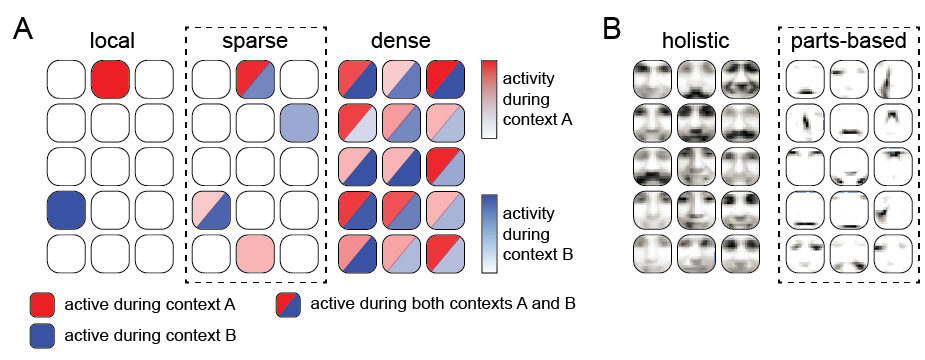
\includegraphics[width=\textwidth]{fig-rev1-sparse}
    \caption{\Acf{NSC} promotes population codes that are both sparse and parts-based.
    \textbf{\emph{A}},
    	   Hypothetical activity in a population of neurons
           during presentation of two different external stimuli (`contexts').
           A sparse code is a trade-off between a local code
           (where a context is represented by the activity of a single neuron,
           and different contexts are represented by different neurons), and a
           dense code (where all neurons are active and their combined activity is
           used to encode each context).
           Dense codes possess great memory capacity, but suffer from cross talk
           among neurons, whereas local codes do not suffer from interference
           but also have no capacity for generalization
           \revise{(inspired by \cite{SpanneJorntell2015})}.
     \textbf{\emph{B}},
           In a holistic representation of faces, 
           individual neurons in the population
           respond themselves to faces as a whole \cite{TanakaFarah1993},
           whereas in a parts-based representation
           individual neurons explicitly encode individual face components
           \cite{Palmer1977},
           such as the eyes, nose, and mouth
           (adapted from \cite{LeeSeung1999} \revise{with permission}).}
	\label{fig:sparse-parts}
\end{figure}


Another approach is to reduce the number of
variables required to represent a particular \revise{input} space;
a process known as
\textbf{dimensionality reduction}.
Dimensionality reduction methods have proved useful in elucidating neural mechanisms
that depend on how the responses of multiple neurons covary,
including odor discrimination in the olfactory system \cite{Broome2006,Koulakov2011}
as well as the selection and integration of sensory inputs 
in the prefrontal cortex \cite{Mante2013}.
% and the ability of premotor cortex 
% to prepare movements without executing them \cite{Kaufman2014}.

In brain areas far removed from sensory input,
neurons typically encode several behaviorally relevant parameters
simultaneously \cite{Rigotti2013,Park2014,PaganRust2014,PougetSejnowski1997},
allowing for multifaceted representations of high-dimensional stimulus spaces.
For example, a population of neurons tasked with encoding human faces
might opt to represent each individual face as a combination of a set of
standard faces (Fig.~\ref{fig:sparse-parts}B, left column).
In such a \textbf{holistic representation} of faces \cite{TanakaFarah1993},
each individual neuron would itself respond to a face as a whole
(i.e., a face `template')
without explicitly representing individual face components,
and an arbitrary face could be represented by 
combining different face templates
(e.g., by adding 10\% of template 1 to 20\% of template 2
and subtracting 30\% of template 3).
On the other hand, faces can also be represented as a combination
of individual face components, such as eyes, noses, and mouth,
in what is known as a \textbf{parts-based representation}
(Fig.~\ref{fig:sparse-parts}B, right column) \cite{Palmer1977}.
Both approaches allow for representing arbitrary faces as a combination of
neural activity, but have drastically different consequences on the
set of stimulus features each neuron responds to.
Although visual information from the eyes, nose, and mouth would of course be
included in a holistic face representation,
that information would not be explicitly represented as structural units
in their own right \cite{TanakaFarah1993}.
Linear combinations of holistic components often involve complex cancellations
between positive and negative contributions,
and thus lack the intuitive meaning of adding parts to form a whole.
In contrast, a parts-based representation allows for only nonsubtractive
combinations of stimulus features \cite{Palmer1977}.
Although the relevant stimulus dimensions are often not known \emph{a priori},
several sophisticated mathematical techniques exist that
allow us to discover these representations directly from experimental data
\cite{Brunton2016,CunninghamYu2014,PillowSimoncelli2006,Sharpee2014,Gao2017,ChangTsao2017}.
In this article, we \revise{suggest} that a variety of neuronal responses
can be understood as an emergent property of efficient population coding
based on dimensionality reduction and sparse coding.
Specifically, we review computational evidence
from data analyses and computer simulations arguing that \ac{NSC}, 
a combination of \textbf{\ac{NMF}}
\cite{PaateroTapper1994,LeeSeung1999} 
and sparse coding,
can generate sparse and parts-based embeddings of
high-dimensional stimulus \revise{and synaptic input} spaces
that resemble \revise{downstream} neuronal population responses in a 
wide variety of brain regions.
This introduces the possibility that \ac{NSC} might be 
\revise{a principle of organization to which many neuronal computations adhere, 
particularly in sensory and association cortices.}
\revise{We furthermore speculate that} \ac{NSC} \revise{may} provide a useful theoretical framework \revise{by} which
to understand the often complex and nonintuitive response properties of neurons
in brain areas far removed from sensory input.
